\documentclass[9pt]{beamer}
\usepackage{tikz}
\usepackage{booktabs}

\definecolor{themecolor}{rgb}{.1, .1, .5}
\definecolor{darkgreen}{rgb}{.1, .1, .5}
\definecolor{myblue}{RGB}{0, 139, 188}

\def \mainroot{../../../}
\input{\mainroot/slides/fthb/local_config.tex}

\mode<presentation>{}
\usefonttheme{structuresmallcapsserif}
\setbeamerfont{footline}{size={\fontsize{10}{12}}}
\setbeamertemplate{footline}[frame number]{}
\setbeamertemplate{navigation symbols}{}

\title{FTHB model slide deck}
\author{Berger, Cui, Turner, and Zwick \\ (DRAFT)}

\def \sdir{stata}
\def \mdir{matlab}


\begin{document}

\begin{frame}
\titlepage
\end{frame}

{
    \setbeamercolor{background canvas}{bg=themecolor}
\frame{
        \Large \color{white} \textbf{Model setup}
    \addtocounter{framenumber}{-1}
}
}

\begin{frame}{Defined parameters}
\textbf{Note:} The entire model is standardized to median household income
 in the 1998-2004 SCF (About ~\$67,000 in 2013 dollars)
\begin{itemize}
        \item $1-\alpha = 0.859:$ Cobb-Douglas parameter, share of expenditure
                in perishable consumption (i.e. $\alpha$ share in durables)
        \item $\gamma = 2:$ Intertemporal elasticity of substitution
        \item $r = 2.4\%:$ rate of return on the safe asset
        \item $r_{borrow} = r + 0.8\%$ interest rate on borrowing (if
                $q \leq (1-\theta)*h*p$)
        \item $\delta = 2.2\%:$ Depreciation rate of hdurable
        \item $F = 6\%:$ total fixed cost on adjusting durable stock
        \item $\underline{s} = 0.8:$ share of the fixed cost borne by the
                seller (i.e. she pays $\underline{s}F$)
        \item $\theta = 20\%$: Required down payment on durable
        \item $\rho_z = 0.91$: Persistence of AR(1) income process
        \item $\sigma_z = 0.20$: S.d. of shocks to income process
        \item $\epsilon = 2.5$: Price elasticity of supply for the representative
               housing firm
\end{itemize}
\end{frame}

\begin{frame}{Calibrated parameters}
        \textbf{Note:} Unlikely that all the parameters below will be
        calibrated.
\begin{itemize}
        \item $\beta = 0.915:$ Discount rate.
        \item $\phi = 0.26\%:$ Rental housing markup (added onto user cost of housing
                yields the rental price as a fraction of housing)
        \item $\phi_{ret} = 0.065\% : $ Rental housing markup in retirement.
        \item $h_{min} = 0.78:$ Minimum size for an owned house (no limits exist on
                renting)
        \item $\Xi = 2.00 :$ A lump sum transfer at retirement equal to a proportion
                of labour income before retirement
        \item $\Psi = 3.60:$ Multiplicative factor on bequest utility (seems large,
               but maybe bequests are also defined differently?)
       \item  $\omega:$ Disutility of rental housing ($=1$ for owned housing)
       \item  $\underline{b}:$ Reference value for bequests: affects marginal
               utility of a unit increase in bequests.
\end{itemize}
\end{frame}

\begin{frame}{Algorithmic details}
\begin{itemize}
        \item Search space over 120 uneven grid points for voluntary equity,
              $q = a + (1-\theta)*h*p$, 90 grid points for $h$
      \item 9 grid points for income process (Tauchen '86 discretization),
              with a range of $\pm 2.5$ the unconditional s.d
              of the AR(1)
      \item  38 working periods, 25 retirement periods. Correspond to ages
              22-84 on data
      \item A steady-state general equilibrium is found by minimizing the
              deviation between the \textbf{average} excess demand for housing
              (see Kaplan, Mitman, Violante, eq. 6) and the average new
              construction supply. \newline
              The minimizing price is found using Brent's method, with
              a liberal convergence threshold. However, the minimum deviation
              still usually reaches less than 1E-2.
\end{itemize}
\end{frame}

{
    \setbeamercolor{background canvas}{bg=themecolor}
\frame{
        \Large \color{white} \textbf{Model in steady-state}
    \addtocounter{framenumber}{-1}
}
}

\begin{frame}{Homeownership over the lifecycle: model v. data}
  \begin{tikzpicture}
       \node
       {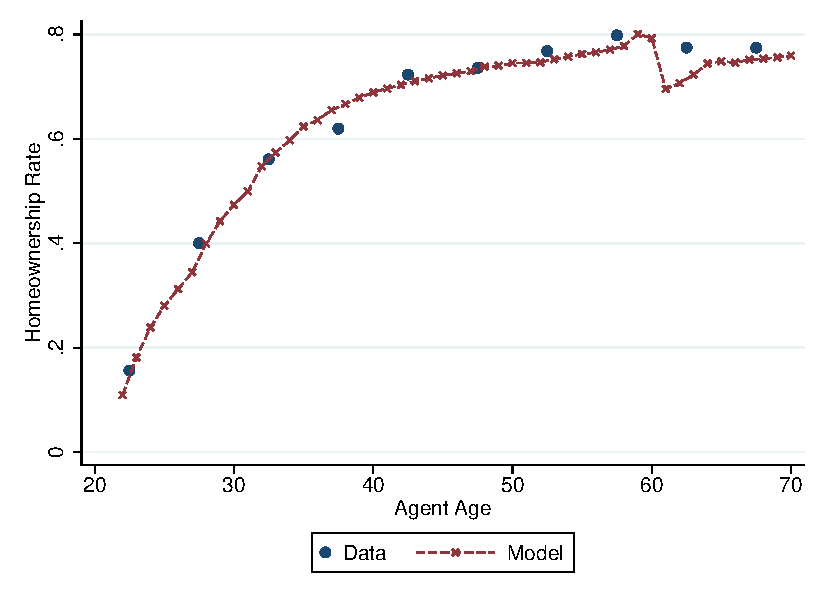
\includegraphics[width=4.4in]{\sdir/fracOwn}};
    \end{tikzpicture}
\end{frame}

\begin{frame}{Assets over the lifecycle: model v. data}

  \begin{tikzpicture}
       \node
       {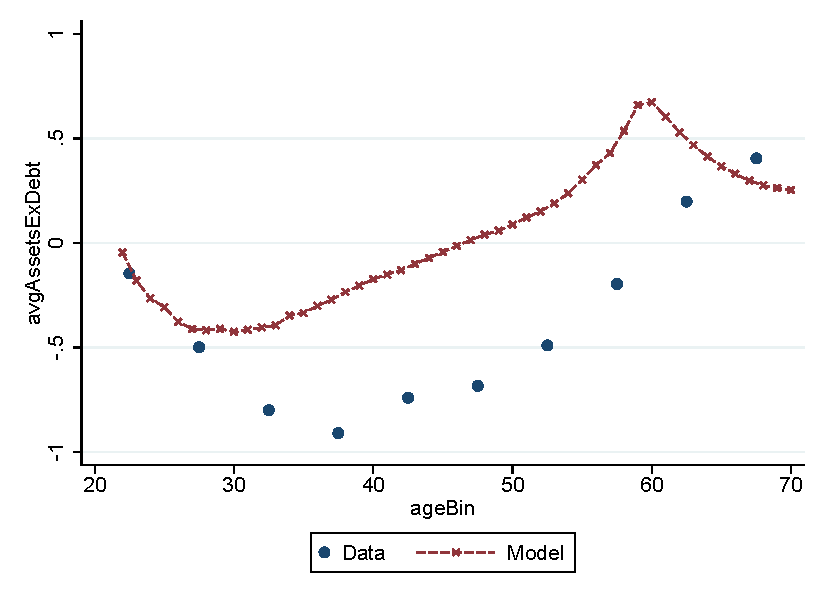
\includegraphics[width=4.4in]{\sdir/avgAssetsExDebt}};
    \end{tikzpicture}
\end{frame}

\begin{frame}{Owned house value over the lifecycle: model v. data}

  \begin{tikzpicture}
       \node
       {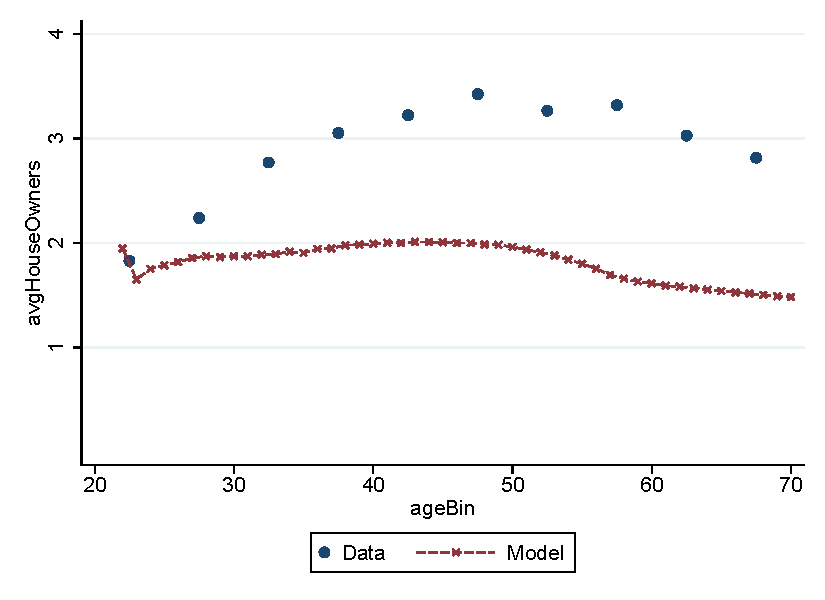
\includegraphics[width=4.4in]{\sdir/avgHouseOwners}};
    \end{tikzpicture}
\end{frame}

\begin{frame}{Distribution of assets for renters, model}
\begin{figure}[pb!]
    \centering
    \begin{tabular}{cc}
    (a) All living renters & (b) Renters of working age \\
    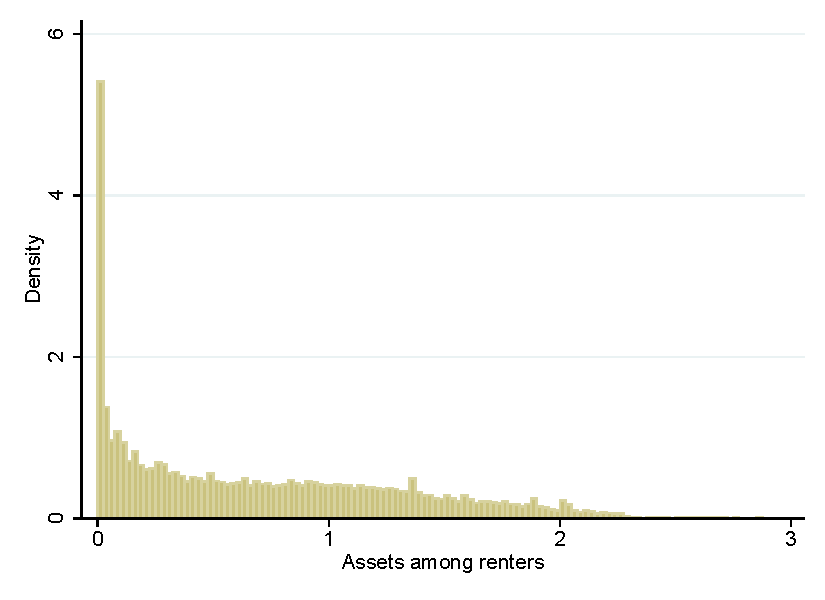
\includegraphics[width=2.1in]{\sdir/rentAssets_model} &
    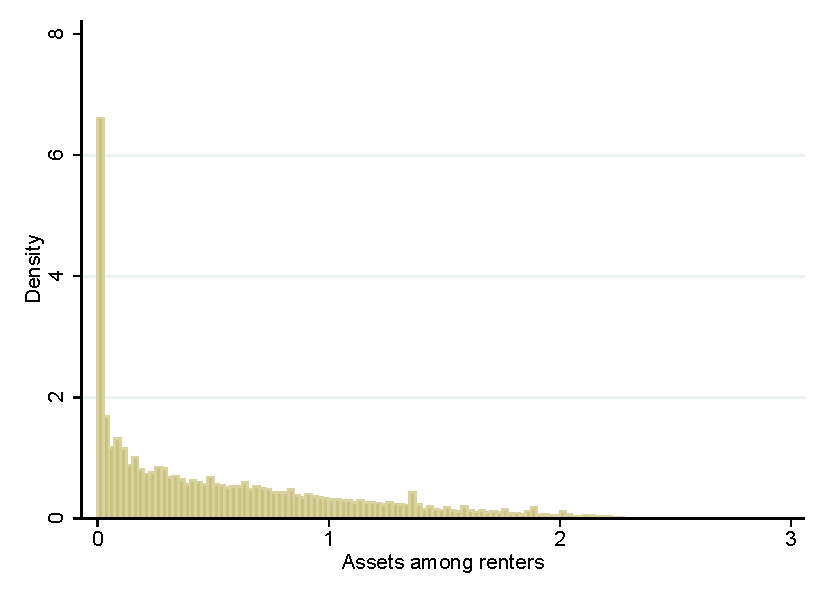
\includegraphics[width=2.1in]{\sdir/rentAssets_workers_model}
    \end{tabular}
\end{figure}
\end{frame}

\begin{frame}{Time series of assets/savings for renters, model}
\begin{figure}[pb!]
    \centering
    \begin{tabular}{cc}
    (a) Median within each age & (b) 75th percentile within each age \\
    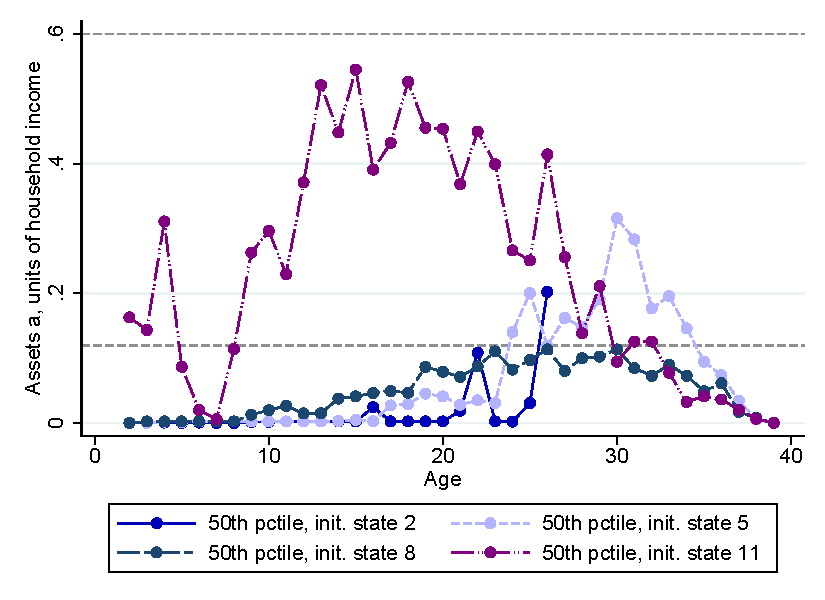
\includegraphics[width=2.1in]{\sdir/asset_race_median} &
    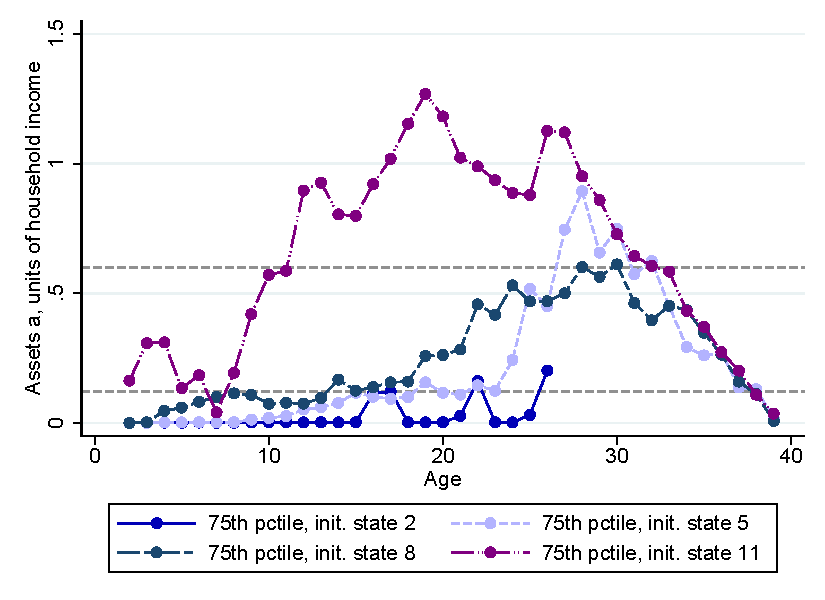
\includegraphics[width=2.1in]{\sdir/asset_race_75p}
    \end{tabular}
\end{figure}
The horizontal lines indicate
\begin{itemize}
        \item The equivalent of \$8,000 in the model;
        \item The average down payment on a house (20\% $\times$ 3 household income units)
\end{itemize}
\end{frame}



\begin{frame}{Distribution of housing/net worth for owners, model}
\begin{figure}[pb!]
    \centering
    \begin{tabular}{cc}
    (a) All living owners & (b) Owners of working age \\
    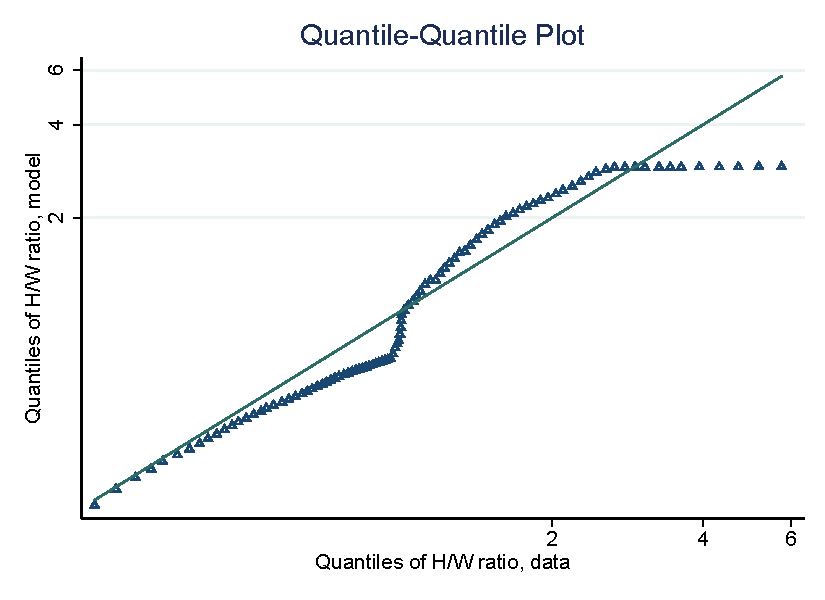
\includegraphics[width=2.1in]{\sdir/ownerWealth_model} &    
    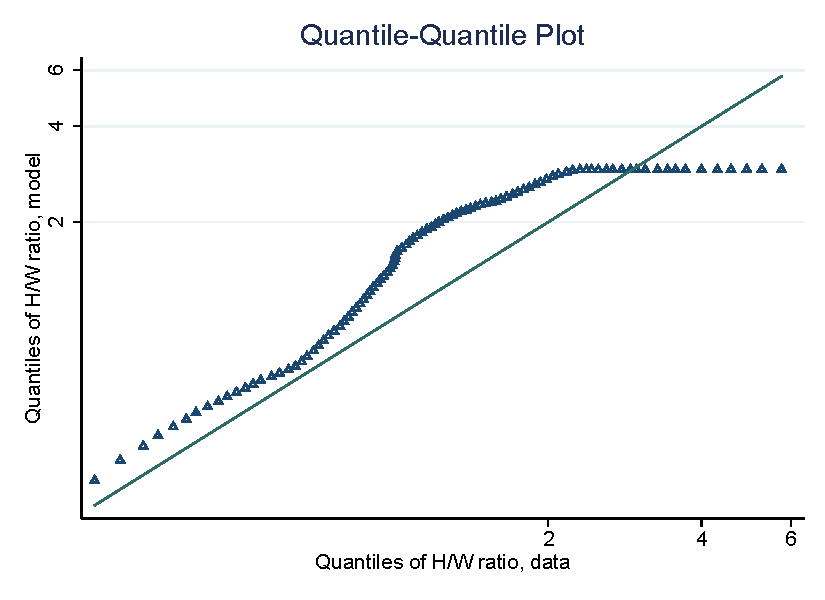
\includegraphics[width=2.1in]{\sdir/ownerWealth_workers_model}
    \end{tabular}
\end{figure}
\end{frame}

\begin{frame}{Lorenz curves for variables in the model}
\begin{figure}[pb!]
    \centering
    \begin{tabular}{cc}
    (a) Owned housing & (b) Net wealth \\
    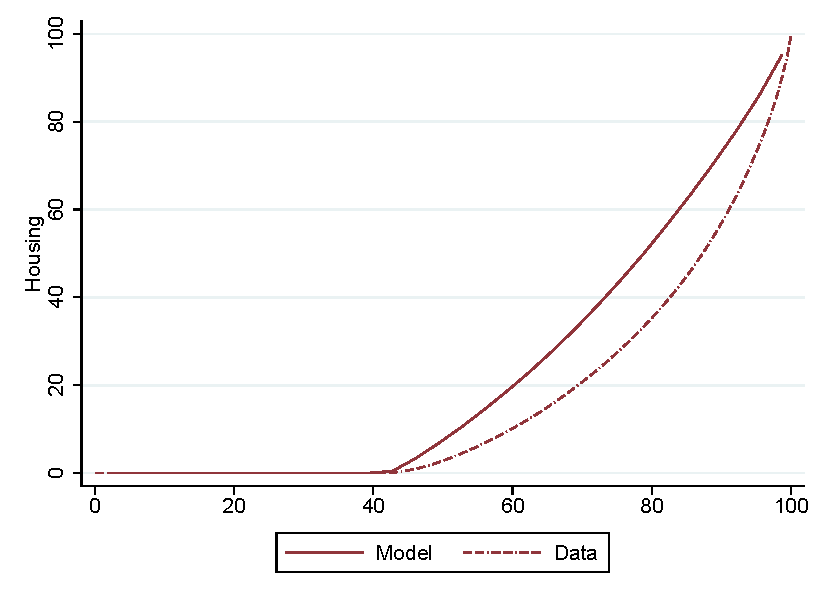
\includegraphics[width=1.8in]{\sdir/houses_dist_model} &
    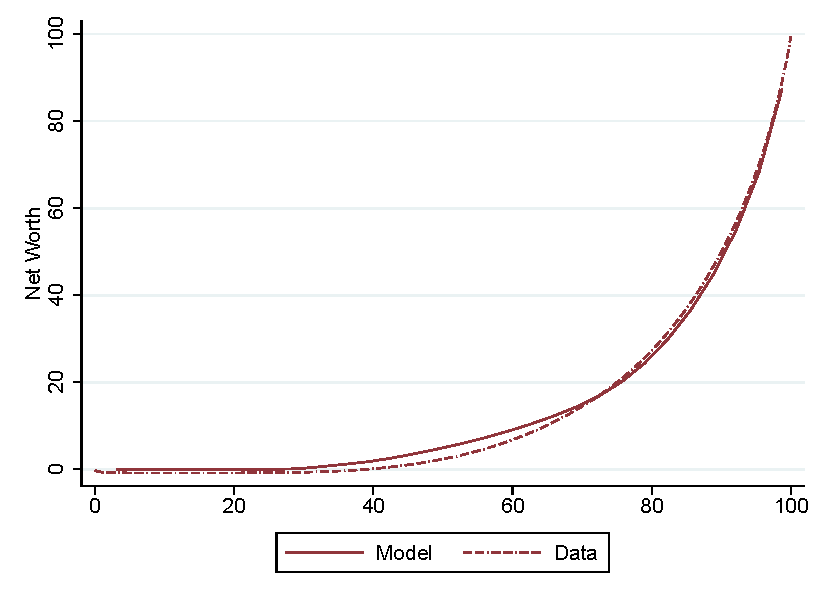
\includegraphics[width=1.8in]{\sdir/networth_dist_model} \\
    \multicolumn{2}{c}{(c) Income in period} \\
    \multicolumn{2}{c}{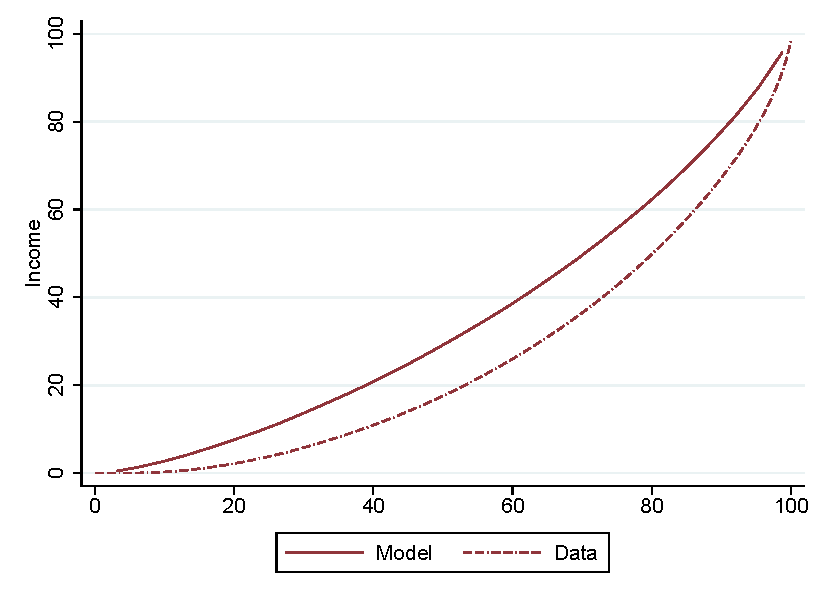
\includegraphics[width=1.8in]{\sdir/income_dist_model}}
    \end{tabular}
\end{figure}
\end{frame}

\begin{frame}{Inequality in housing: model v. data}
\begin{figure}[pb!]
    \centering
    \begin{tabular}{cc}
    (a) Lorenz curves from SCF data & (b) Lorenz curves from model panel \\
    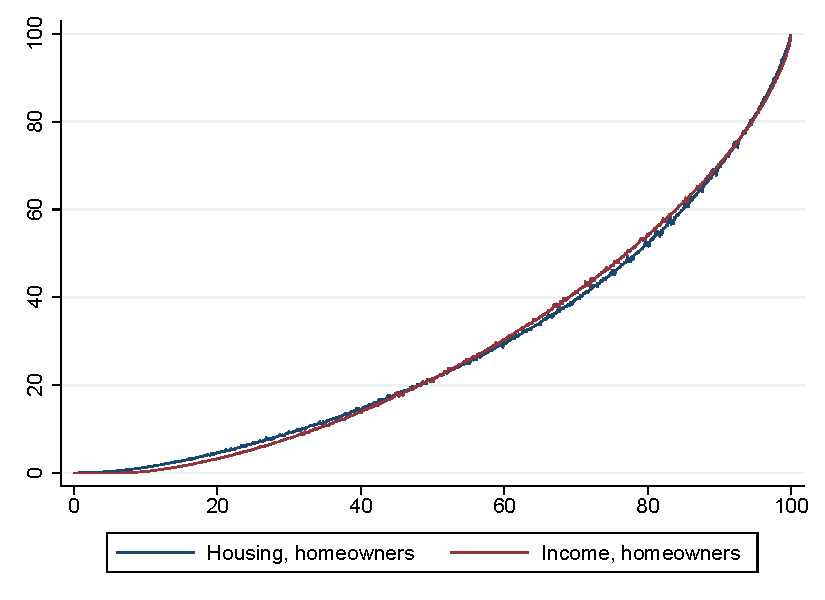
\includegraphics[width=2.1in]{\sdir/wealthDist_data} &
    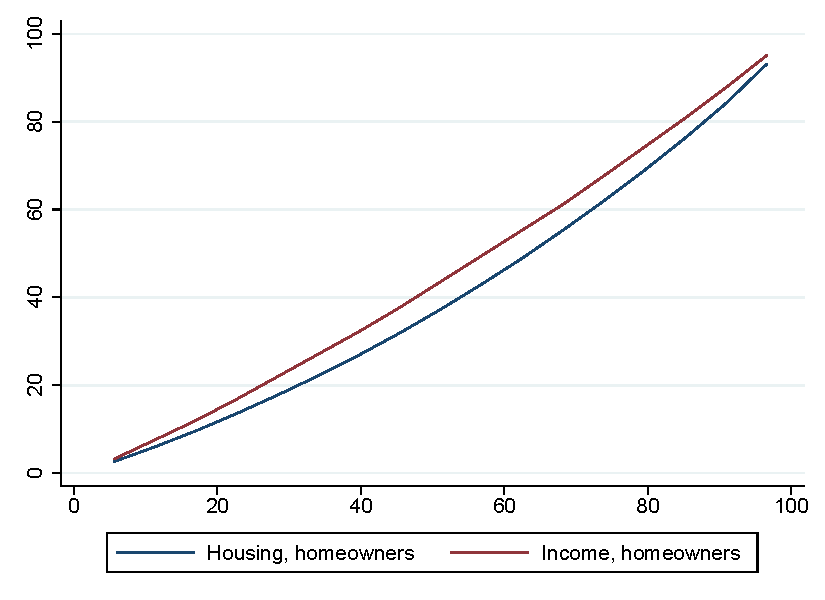
\includegraphics[width=2.1in]{\sdir/wealthDist_model}
    \end{tabular}
\end{figure}
\end{frame}

\begin{frame}{Distribution of First-Time Homebuyers: model v. data}
\begin{figure}[pb!]
    \centering
    \begin{tabular}{c}
    %(a) Estimated distribution from IRS data \\
    %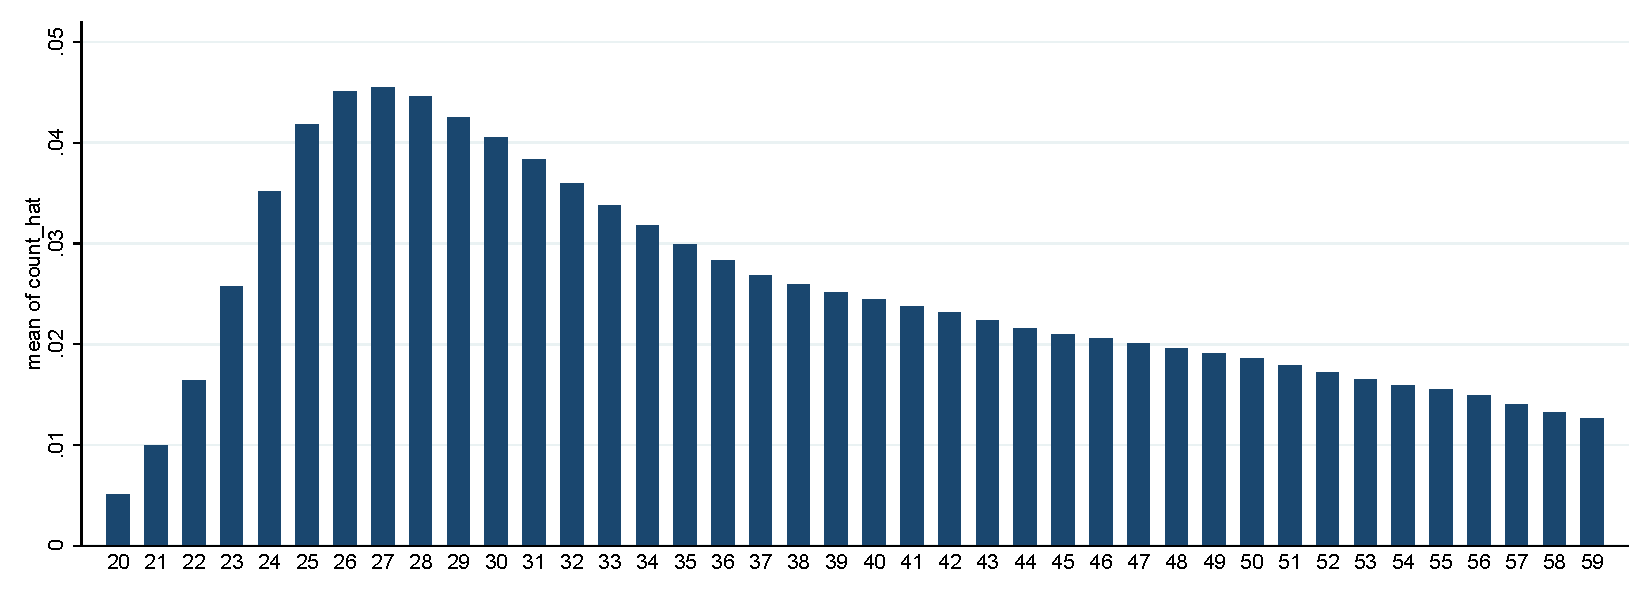
\includegraphics[width=2.1in]{\sdir/EZ_FTHBdist} \\
    %(b) Distribution from model panel \\
    \vspace*{3in}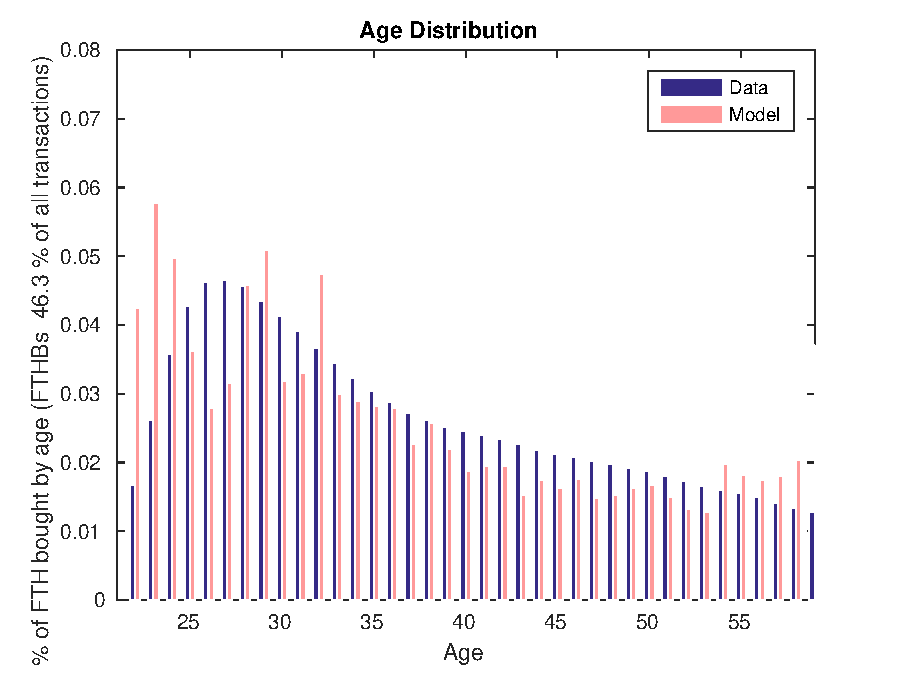
\includegraphics[width=4.2in]{\mdir/fracFthb}
    \end{tabular}
\end{figure}
\end{frame}

\begin{frame}{Upscaling of housing for FTHBs, model}

  \begin{tikzpicture}
       \node
       {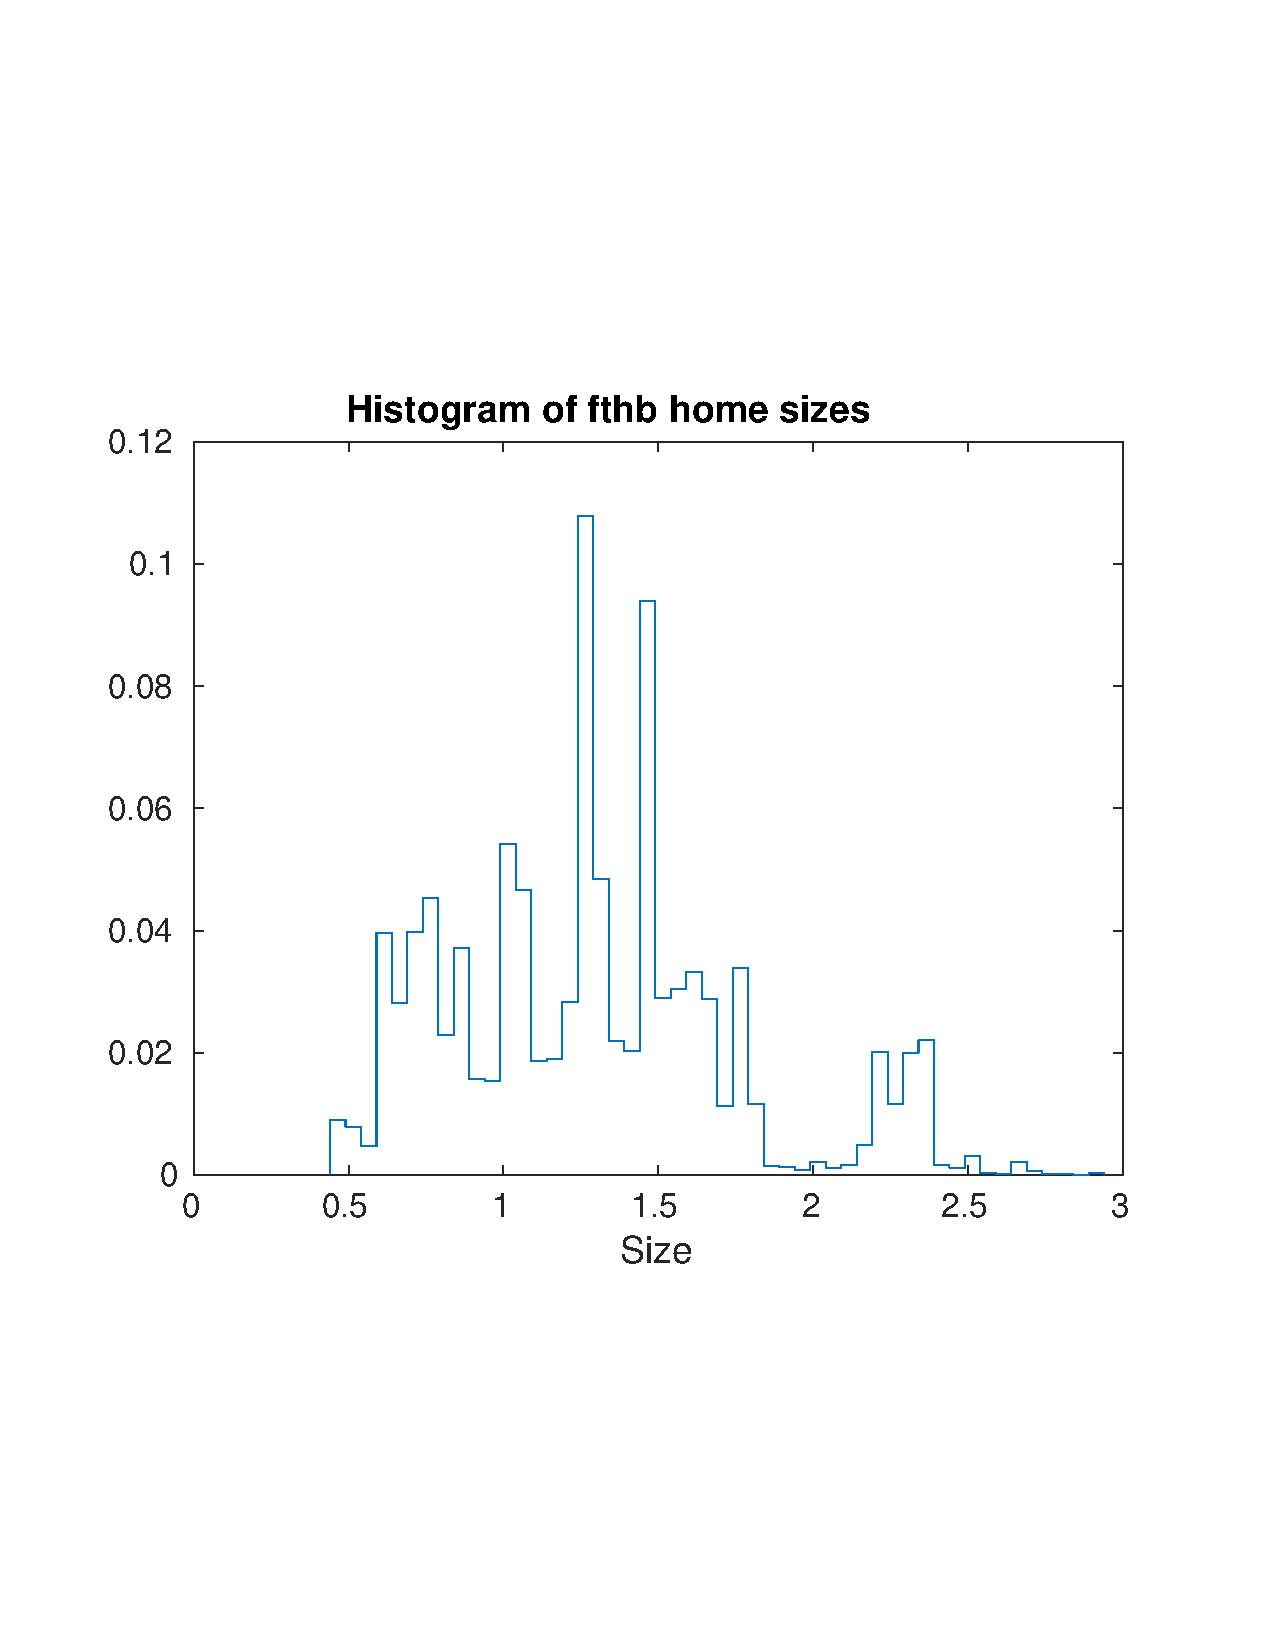
\includegraphics[width=4.4in]{\mdir/HouseSize}};
    \end{tikzpicture}
\end{frame}

{
    \setbeamercolor{background canvas}{bg=themecolor}
\frame{
        \Large \color{white} \textbf{Policy effects, exogenous prices}
    \addtocounter{framenumber}{-1}
}
}

\begin{frame}{Policy specifications}

\begin{itemize}
        \item Every policy assumes the price is unchanged from the steady-state
                equilibium price (so effects are exaggerated in magnitude)
        \item Policy 1 (first five slides) is a policy where, if the credit is
                claimed, the equivalent of \$8,000 is inapplicable toward the
                down payment, but received the period after the purchase
                (this is trying to emulate the FTHB credit)
        \item Policy 2 is a policy where the \$8,000 is
               rebated on the down payment of the house, and nothing
              else (this is counterfactual)
        \item Policy 3 is a policy like Policy 1, except the subsidy is
              much smaller (more like \$6.50). It verifies effects aren't
              large in the first two policies due to bugs.

\end{itemize}

\end{frame}


\begin{frame}{Time series of variables during transition period (1)}

  \begin{tikzpicture}
       \node
       {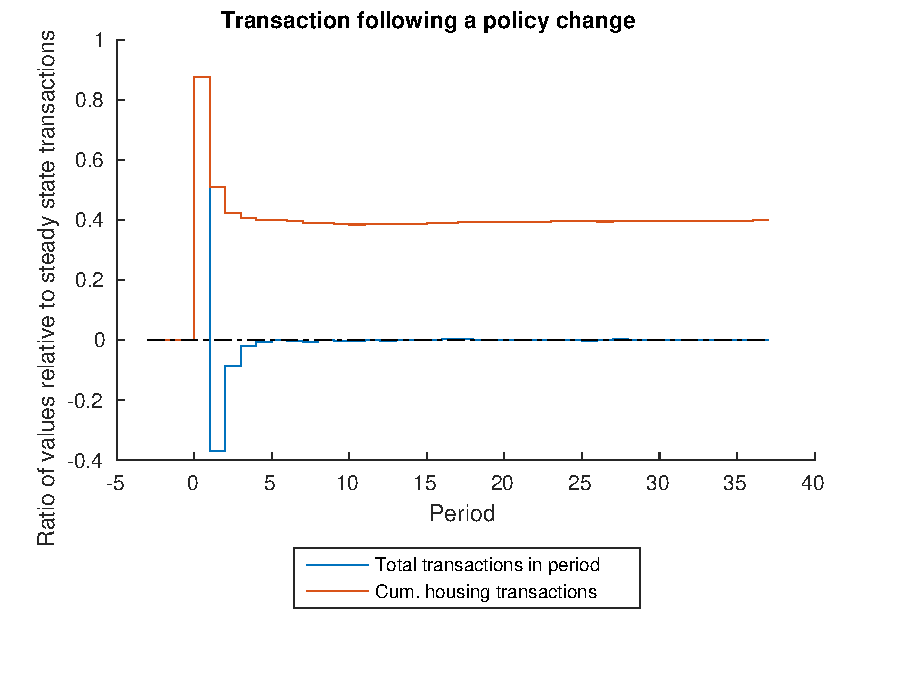
\includegraphics[width=4.4in]{\mdir/FTHB/FthbShock_experiment_monetary_nodown}};
    \end{tikzpicture}
\end{frame}

\begin{frame}{Policy-induced shifts in FTHB age distribution (1)}

  \begin{tikzpicture}
       \node
       {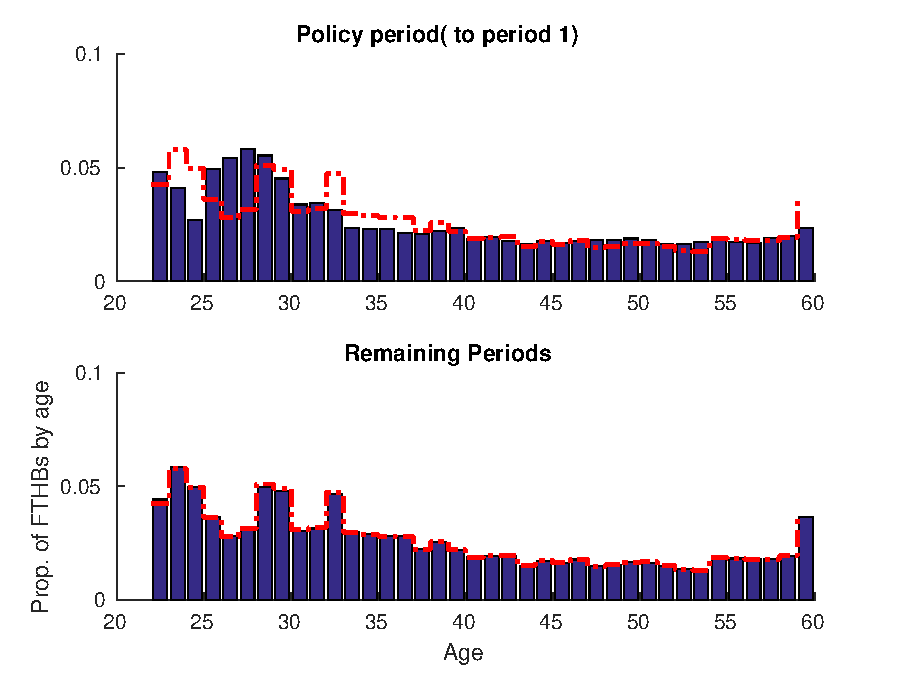
\includegraphics[width=4.4in]{\mdir/FTHB/FthbShockAge_experiment_monetary_nodown}};
    \end{tikzpicture}
\end{frame}

\begin{frame}{Policy-induced shifts in house size (1)}

  \begin{tikzpicture}
       \node
       {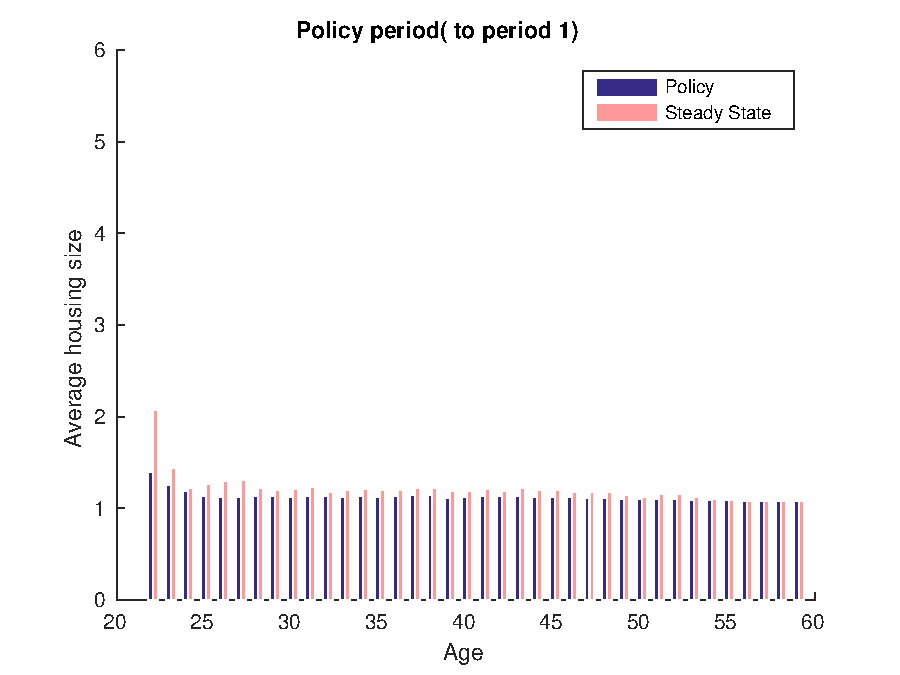
\includegraphics[width=4.4in]{\mdir/FTHB/HouseInvShockAge_experiment_monetary_nodown}};
    \end{tikzpicture}
\end{frame}

\begin{frame}{Heatmap of FTHB housing wealth-consumption ratio (1)}

  \begin{tikzpicture}
       \node
       {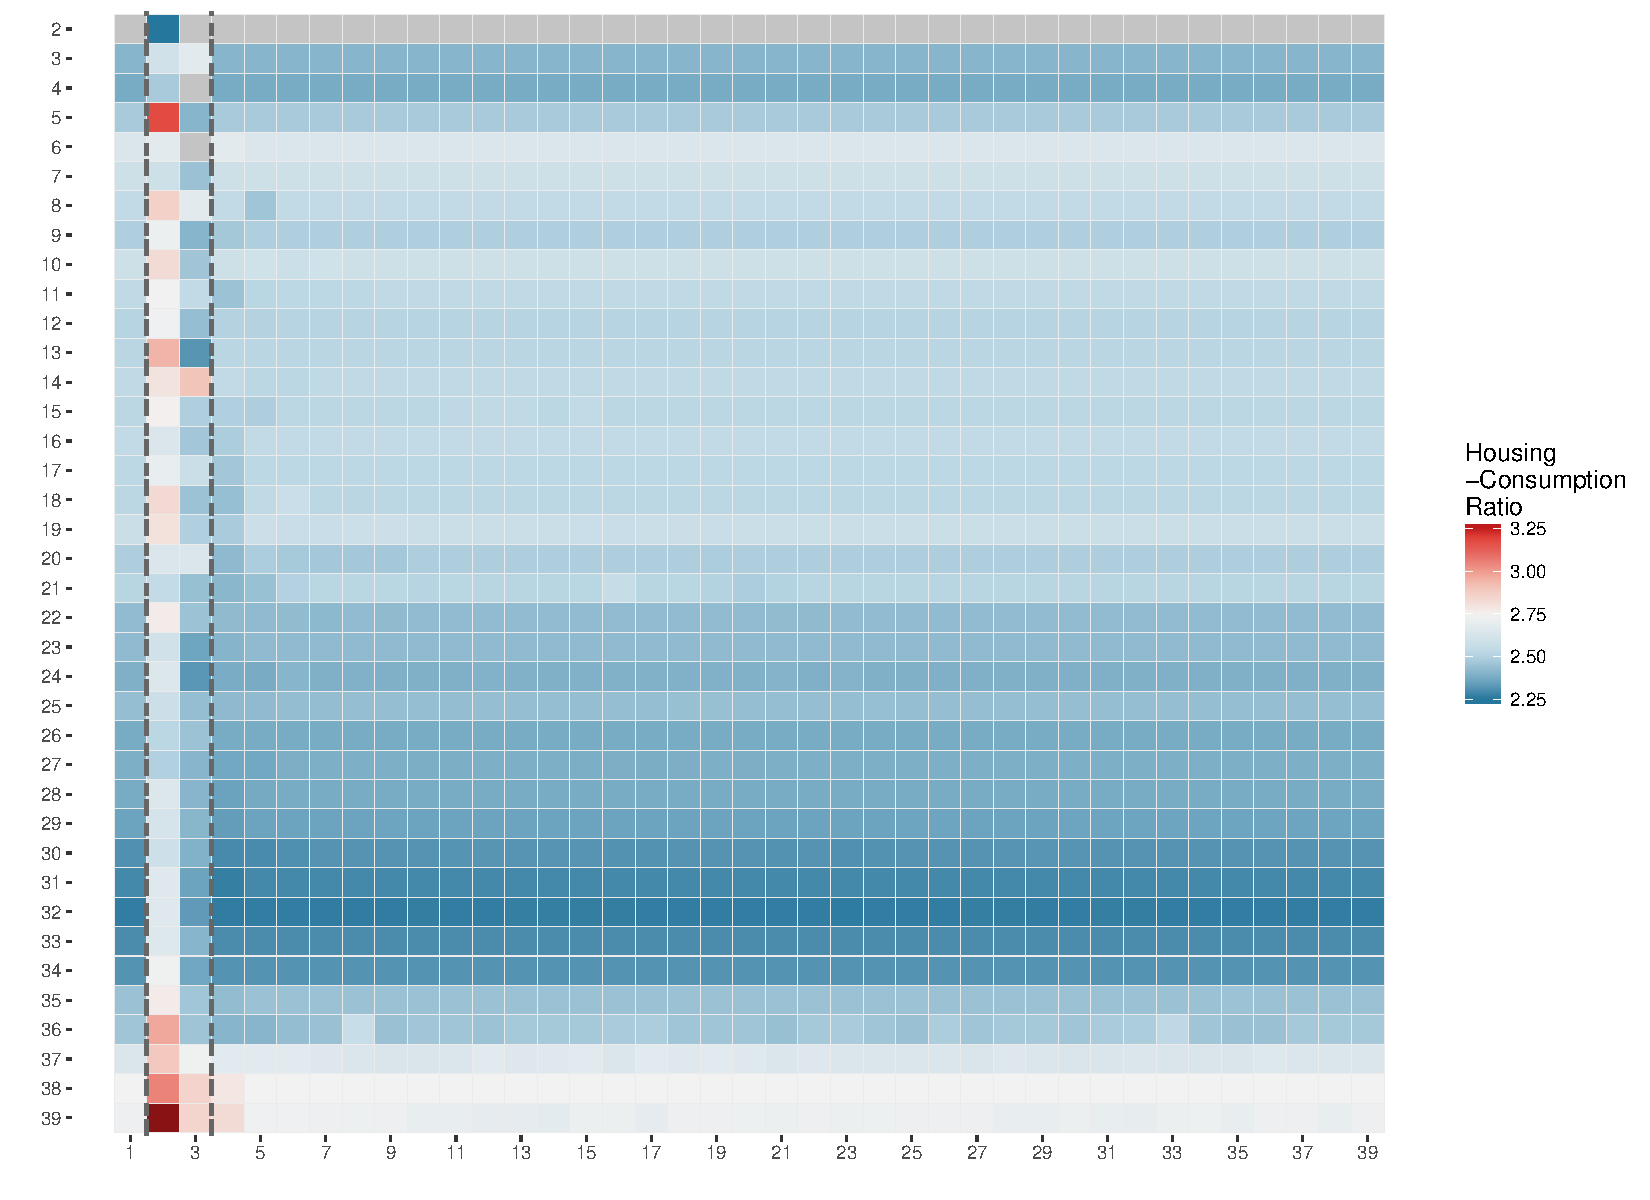
\includegraphics[width=4.4in]{\sdir/heatmap_h}};
    \end{tikzpicture}
\end{frame}

\begin{frame}{Heatmap of FTHB financial assets before purchase (1)}

  \begin{tikzpicture}
       \node
       {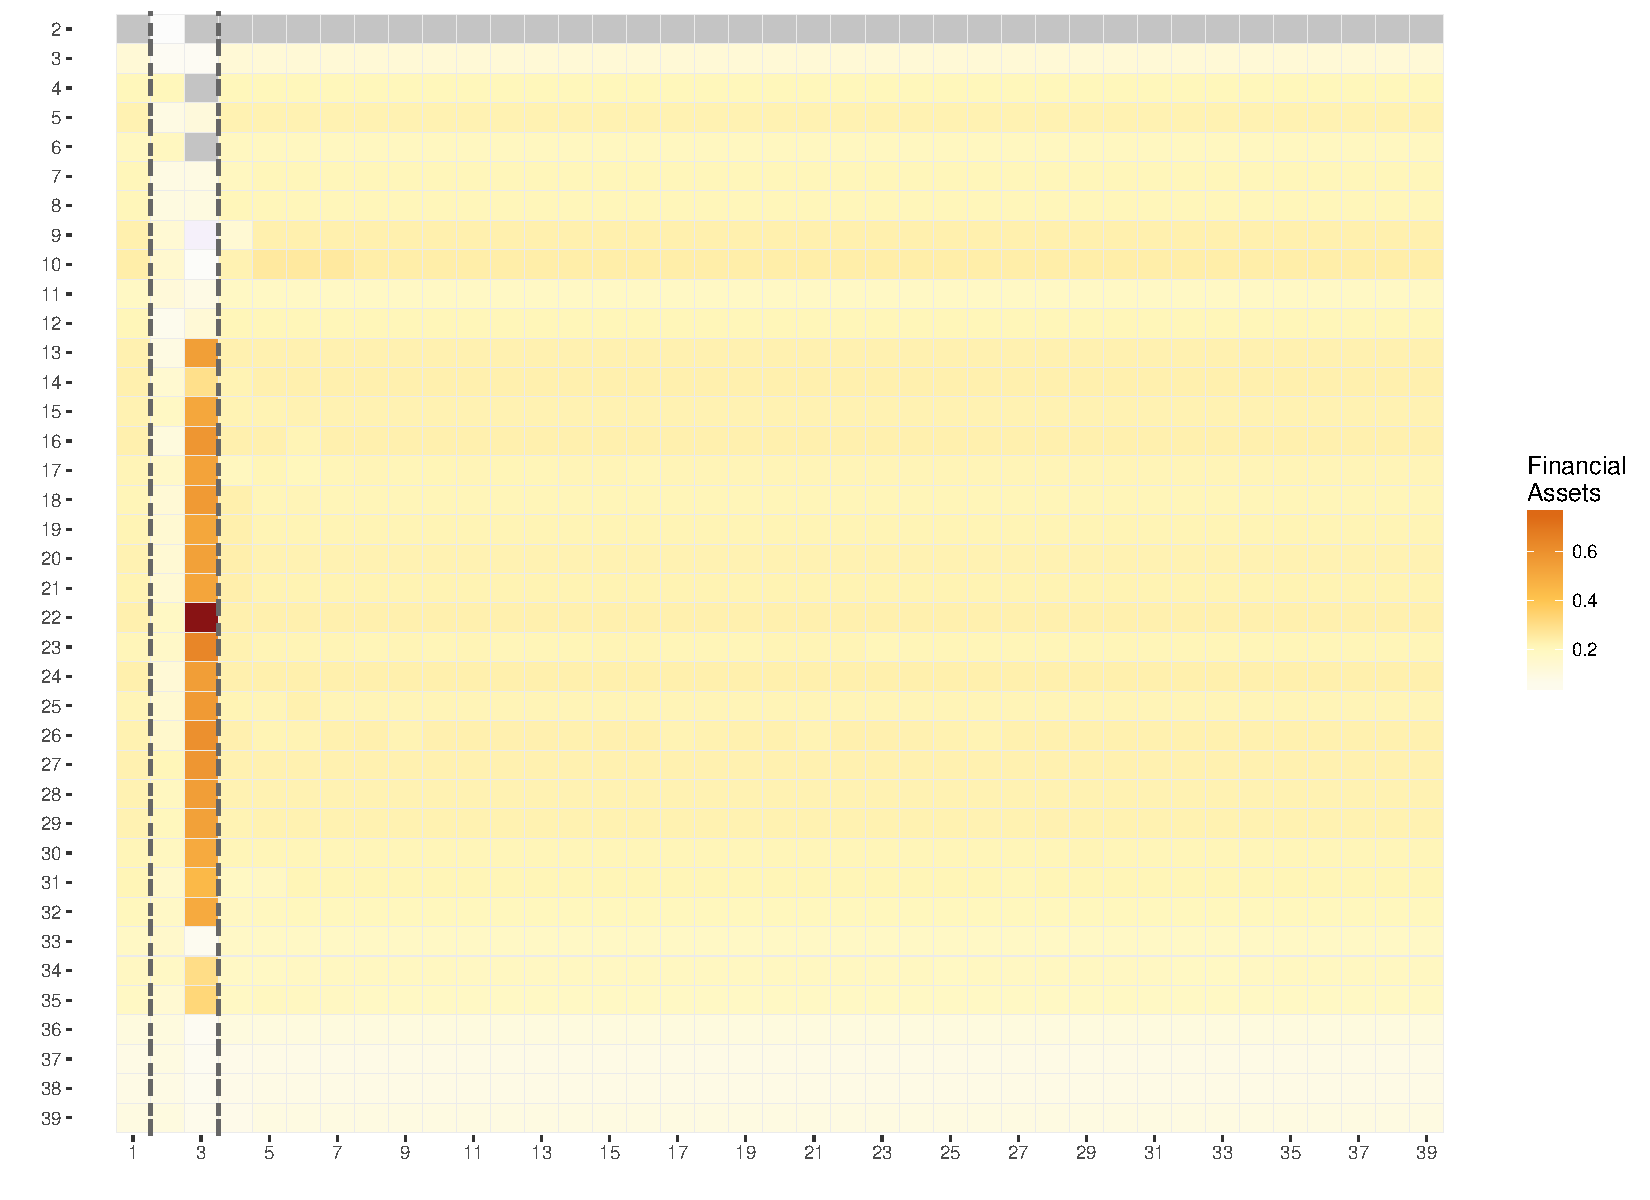
\includegraphics[width=4.4in]{\sdir/heatmap_a}};
    \end{tikzpicture}
\end{frame}



\begin{frame}{Time series of variables during transition period (2)}

  \begin{tikzpicture}
       \node
       {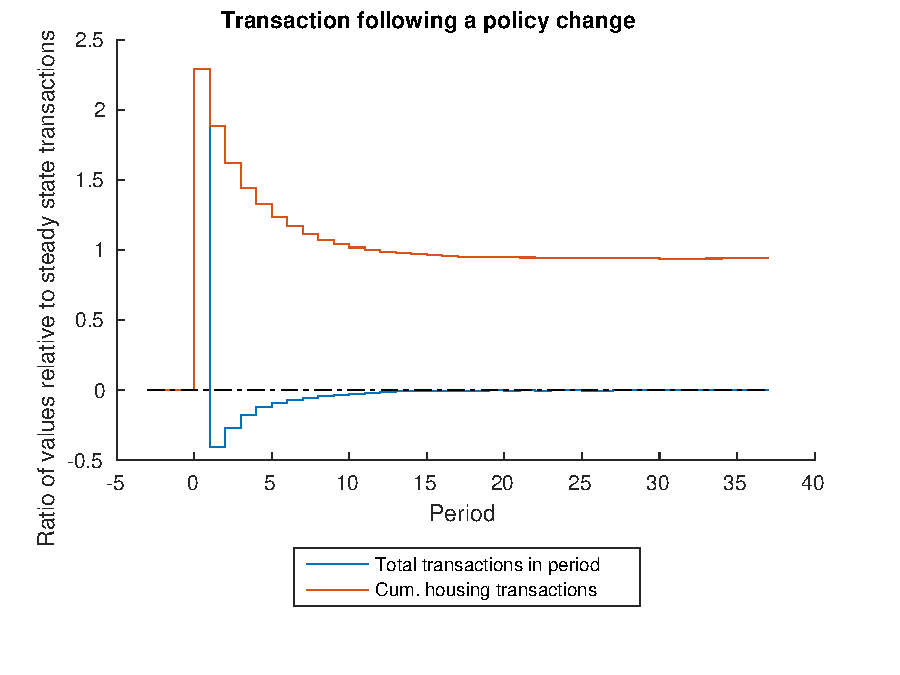
\includegraphics[width=4.4in]{\mdir/FTHB/FthbShock_experiment_monetary}};
    \end{tikzpicture}
\end{frame}

\begin{frame}{Policy-induced shifts in FTHB age distribution (2)}

  \begin{tikzpicture}
       \node
       {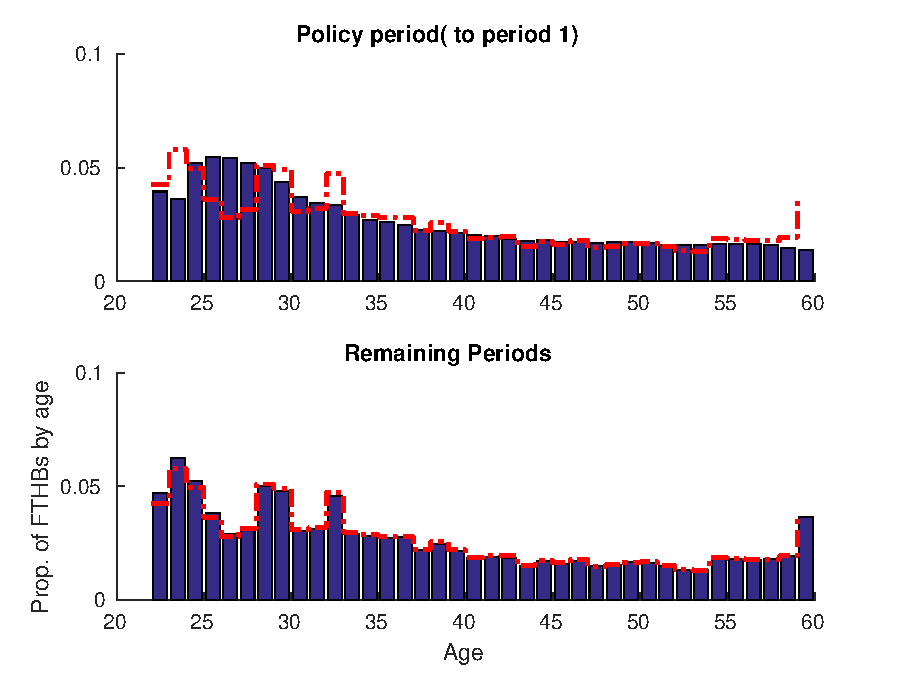
\includegraphics[width=4.4in]{\mdir/FTHB/FthbShockAge_experiment_monetary}};
    \end{tikzpicture}
\end{frame}

\begin{frame}{Policy-induced shifts in house size (2)}

  \begin{tikzpicture}
       \node
       {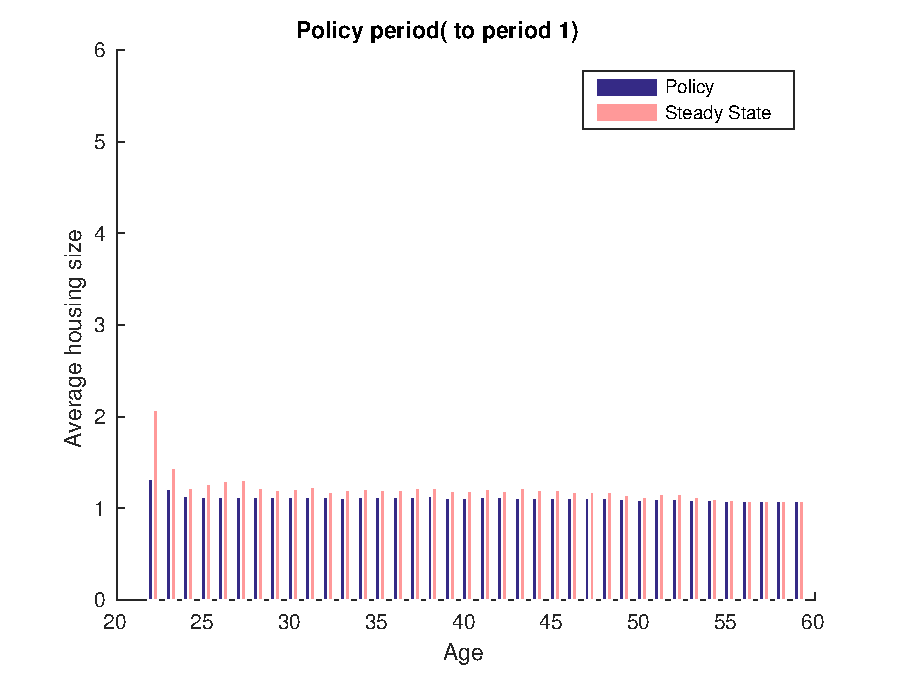
\includegraphics[width=4.4in]{\mdir/FTHB/HouseInvShockAge_experiment_monetary}};
    \end{tikzpicture}
\end{frame}

\begin{frame}{Time series of variables during transition period (3)}

  \begin{tikzpicture}
       \node
       {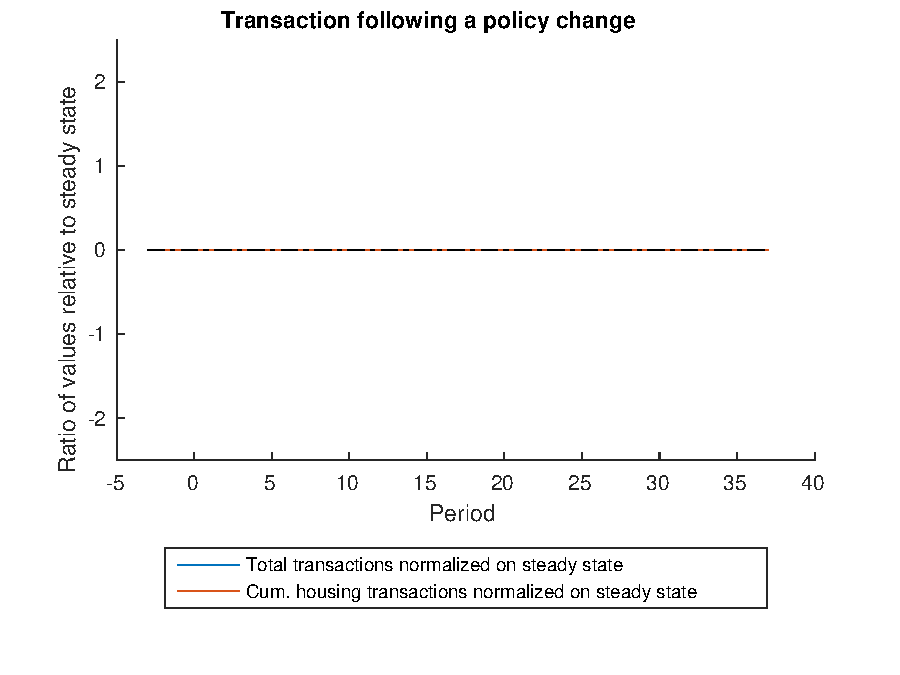
\includegraphics[width=4.4in]{\mdir/FTHB/FthbShock_experiment_monetary_little}};
    \end{tikzpicture}
\end{frame}

\begin{frame}{Policy-induced shifts in FTHB age distribution (3)}

  \begin{tikzpicture}
       \node
       {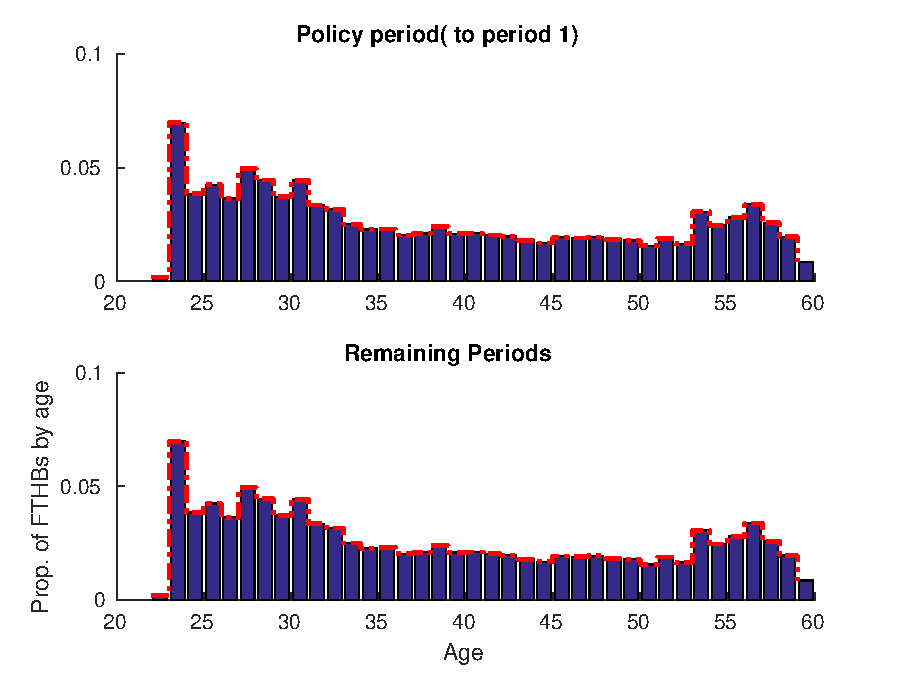
\includegraphics[width=4.4in]{\mdir/FTHB/FthbShockAge_experiment_monetary_little}};
    \end{tikzpicture}
\end{frame}

\begin{frame}{Policy-induced shifts in house size (3)}

  \begin{tikzpicture}
       \node
       {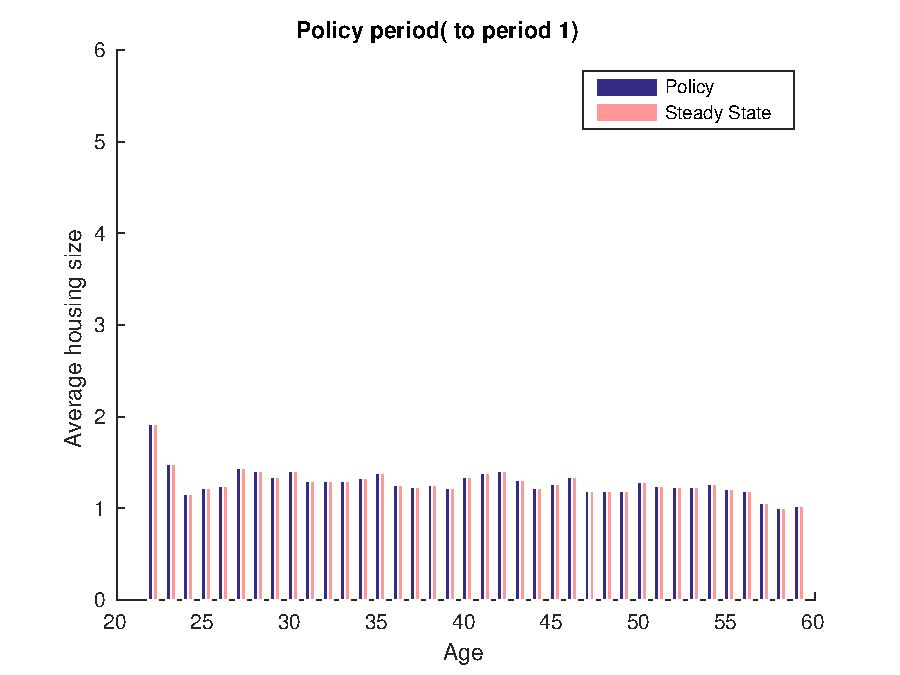
\includegraphics[width=4.4in]{\mdir/FTHB/HouseInvShockAge_experiment_monetary_little}};
    \end{tikzpicture}
\end{frame}

\begin{frame}{Heatmap of FTHB housing wealth-consumption ratio (3)}

  \begin{tikzpicture}
       \node
       {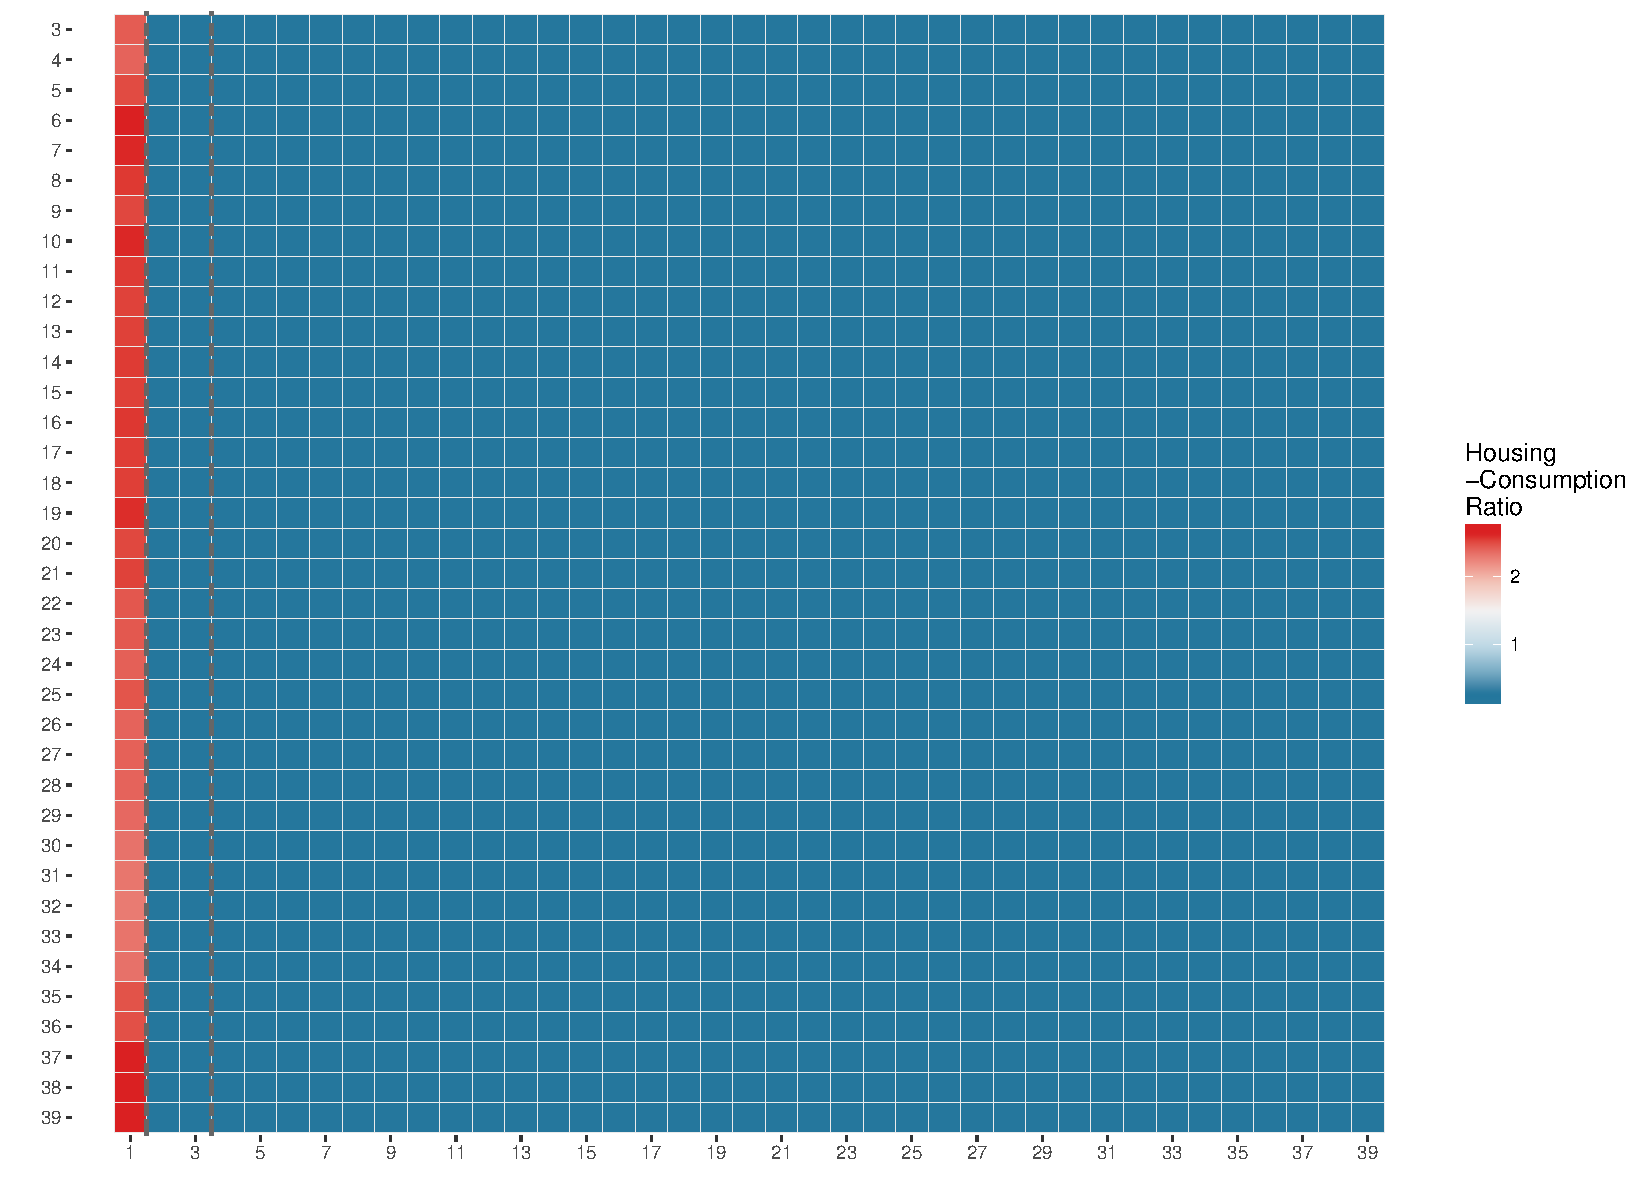
\includegraphics[width=4.4in]{\sdir/heatmap_h_little}};
    \end{tikzpicture}
\end{frame}

\begin{frame}{Heatmap of FTHB financial assets before purchase (3)}

  \begin{tikzpicture}
       \node
       {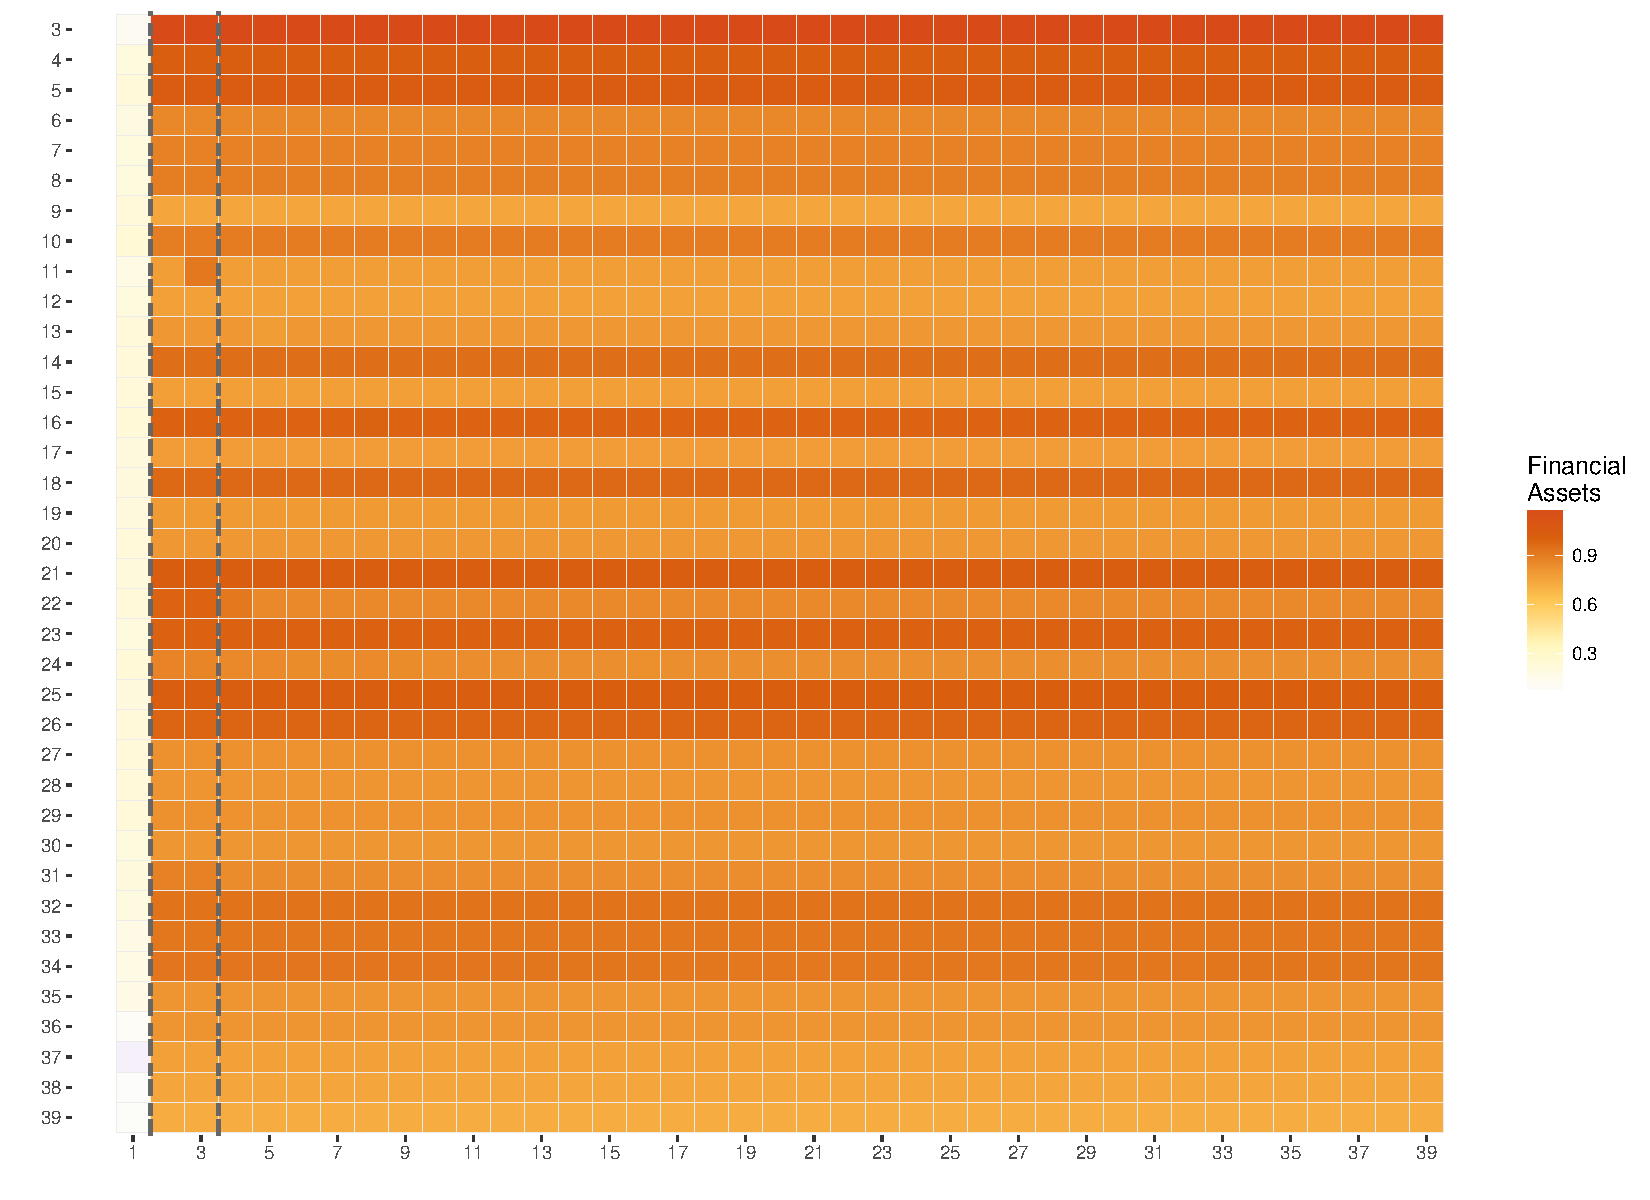
\includegraphics[width=4.4in]{\sdir/heatmap_a_little}};
    \end{tikzpicture}
\end{frame}



\begin{frame}{Counterfactual binscatters for induced FTHBs}

\end{frame}

\end{document}
